\documentclass[notitlepage]{report}

\usepackage{etoolbox}
\patchcmd{\thebibliography}{\chapter*}{\section*}{}{}

\title{A Quantum \texttt{popcount} Circuit for Sieving}
\author{Martin R.~Albrecht, Eamonn W.~Postlethwaite}
\date{\today}

\usepackage{amsmath}
\usepackage{amsfonts}
\usepackage{amssymb}

\usepackage{braket}
\usepackage{subcaption}
\usepackage{graphicx}

\usepackage{array}
\usepackage{booktabs}
\renewcommand{\arraystretch}{1}

\usepackage{tikz}

\usepackage{algorithm}
\usepackage{algpseudocode}

\usepackage{amsthm}
\newtheorem*{thm}{Theorem}
\newtheorem*{lem}{Lemma}
\theoremstyle{definition}
\newtheorem*{mydef}{Definition}
\newtheorem*{heu}{Heuristic}

\usepackage{geometry}

\begin{document}

\maketitle

Using the adder of~\cite{cuccaro2004new} we build a reversible circuit that takes as input bitstring representatives of two lattice vectors, takes a bitwise \texttt{CNOT}, determines the Hamming weight of the outcome and further determines whether this Hamming weight is greater than some bound.
This exact operation is the most frequently used operation in state of the art lattice sieving techniques.

Throughout qubits $a_{i}$ are ancillae and are initialised as $\ket{0}$, the $v_{i}, w_{i} \in \{0, 1\}, i \in \{0, \dots, d - 1\}$ form the bitstring representatives of lattice vectors $v, w$.
These are calculated as the signs of the entries of $v$ and $w$, i.e.~a negative entry is mapped to $0$ and a positive or zero entry to $1$.
This provides a lossy sketch of the lattice vectors under consideration.
The \texttt{CNOT} gate is written as \texttt{CNOT}$(x, y) = (x, x \oplus y)$.
The gates labelled \texttt{add} are the optimised adder of~\cite{cuccaro2004new}.
To sum two $\ell$ bit numbers, this gate \texttt{add} takes $2\ell + 2$ inputs, the topmost and bottommost are ancillae and those inbetween are the interleaved bits of the numbers to be added.
More precisely let $x = x_{\ell-1}\dots x_{0}$ and $y = y_{\ell-1}\dots y_{0}$ be two numbers to be added represented in binary, then \texttt{add}$(a_{0}, x_{0}, y_{0}, \dots, x_{\ell-1}, y_{\ell-1}, a_{1}) = (a_{0}, s_{0}, y_{0}, \dots, s_{\ell-1}, y_{\ell-1}, s_{\ell})$ with $s_{i}$ as bit $i$ of the sum.
In particular the first ancillary remains $\ket{0}$ but the second contains the final carry.
We need some number, linear in $d$, of the \texttt{add} gates described above.

The notation $s^{i\dots j}_{k}$ in Figure~\ref{fig:naive_popcnt} denotes bit $k$ of the sum (over the integers)
\[
    \displaystyle\sum\limits_{l=i}^{j}{v_{l} \oplus w_{l}}.
\]
Finally the \texttt{OR} gate in Figure~\ref{subfig:naive_popcnt3} consumes an ancillary, \texttt{OR}$(a, x, y) = (a \oplus (xy), x\vee y, y)$.

A reduction between $v$ and $w$ is likely if the sum of the $v_{i} \oplus w_{i}$ is less than some bound, here $2^{k}, k \in \mathbb{Z}_{\geq 1}$.
Let the bit length of this sum be $n = \lfloor\log_{2}d\rfloor + 1$.
We therefore take a (non exclusive) \texttt{OR} over the $n - k$ high bits of the sum and reject pair $(v, w)$ for further testing if we receive a $\ket{1}$.
We require some number, linear in $n$, of the \texttt{OR} gates described above.
An example with $d = 4, k = 1$ is given in Figure~\ref{fig:naive_popcnt}.

\begin{figure}
    \begin{subfigure}{.3\textwidth}
        \centering
        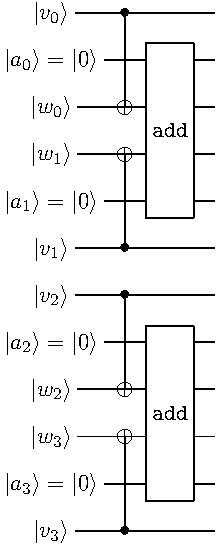
\includegraphics{popcnt_sieve_pt1}
        \caption{The \texttt{CNOT}s and the first round of addition.}\label{subfig:naive_popcnt1}
    \end{subfigure}
    \dots
    \begin{subfigure}{.3\textwidth}
        \centering
        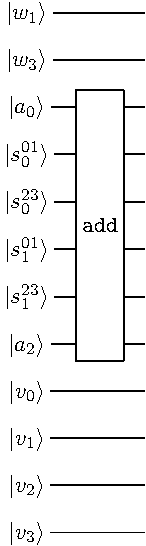
\includegraphics{popcnt_sieve_pt2}
        \caption{Another round of addition.}\label{subfig:naive_popcnt2}
    \end{subfigure}
    \dots
    \begin{subfigure}{.3\textwidth}
        \centering
        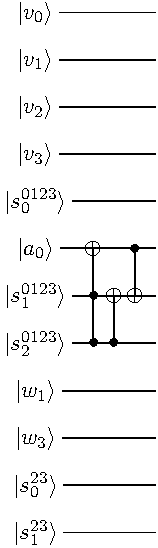
\includegraphics{popcnt_sieve_pt3}
        \caption{An \texttt{OR}, the centre qubit of the three determines the outcome.}\label{subfig:naive_popcnt3}
    \end{subfigure}
    \caption{A simple quantum circuit for determining whether a specific \texttt{popcount} is greater than a given bound.}\label{fig:naive_popcnt}
\end{figure}

We require at most $d$ ancillae as inputs to the \texttt{add} gates, with one definitely remaining in the state $\ket{0}$. Furthermore, letting $n' = \lceil (n - k)/2\rceil$ we require $2n' - 1$ \texttt{OR} gates and hence $2n' - 2$ further ancillae. In terms of $d$ this is $d + O(\log_{2}d)$ ancillae. The width of the circuit is therefore $3d + O(\log_{2}d)$, $2d$ of which represents $v, w$.

The $d$ \texttt{CNOT}s require\dots\ $d$ \texttt{CNOT} gates.
There are $d/2^{i}$ \texttt{add} gates which add two $i$ bit numbers together, for $i \in \{1, \dots, \lceil \log_{2}d\rceil\}$. Each has a number, linear in $i$, of \texttt{Toffoli} and \texttt{CNOT} gates. Therefore the number of such gates required is $O(d)$.
The $2n' - 1$ \texttt{OR} gates require $4n' - 2$ \texttt{CNOT}s and $2n' - 1$ \texttt{Toffoli} gates, or $O(\log_{2}d)$ of both.
In total the circuit has $O(d)$ \texttt{CNOT} and \texttt{Toffoli} gates.

The depth of the circuit is $O\left({(\log_{2}d)}^{2}\right)$.

The adder circuit chosen here uses two ancillae but has linear depth in the bit length, $n$, of the numbers being added. There exist~\cite{Takahashi:2008:FQC} quantum adders which match the depth, $O(\log n)$, of the asymptotically optimal classical adders, but however require $O(n/\log n)$ ancillae. The choice made here simply follows~\cite{SHA2} but could just as easily not.

\bibliographystyle{alpha}
\bibliography{local}

\end{document}
